\subsection{Pressione}

Variamo la pressione nella camera tenendo la sorgente a \SI{0}{\degree} per cercare in quali condizioni l'aria residua non influisce sulla misura.
Registriamo per ogni valore della pressione il rate di eventi ed il relativo spettro. In \autoref{tab:press} sono presenti i dati ed in \autoref{fig:press} il loro andamento.

Dal grafico di \autoref{fig:press} non si nota nessuna variazione dei conteggi fino a $\sim\SI{500}{mbar}$,
ma lo spettro inizia a spostarsi verso il basso già a $\sim\SI{10}{mbar}$.
Questo risultato ci assicura una grande indipendenza dalla condizione di vuoto della camera, soprattutto durante le misure notturne. In tale periodo della giornata è vietato tenere la pompa accesa e, come abbiamo potuto verificare, la pressione risale fino al mbar anche dopo due giorni dalla chiusura della pompa. Quindi possiamo tranquillamente fare misure di lunga durata.
Come atteso la distribuzione di energia delle particelle $\alpha$ si allarga
quando la perdita di energia in aria diventa significativa.

\begin{figure}
\centering
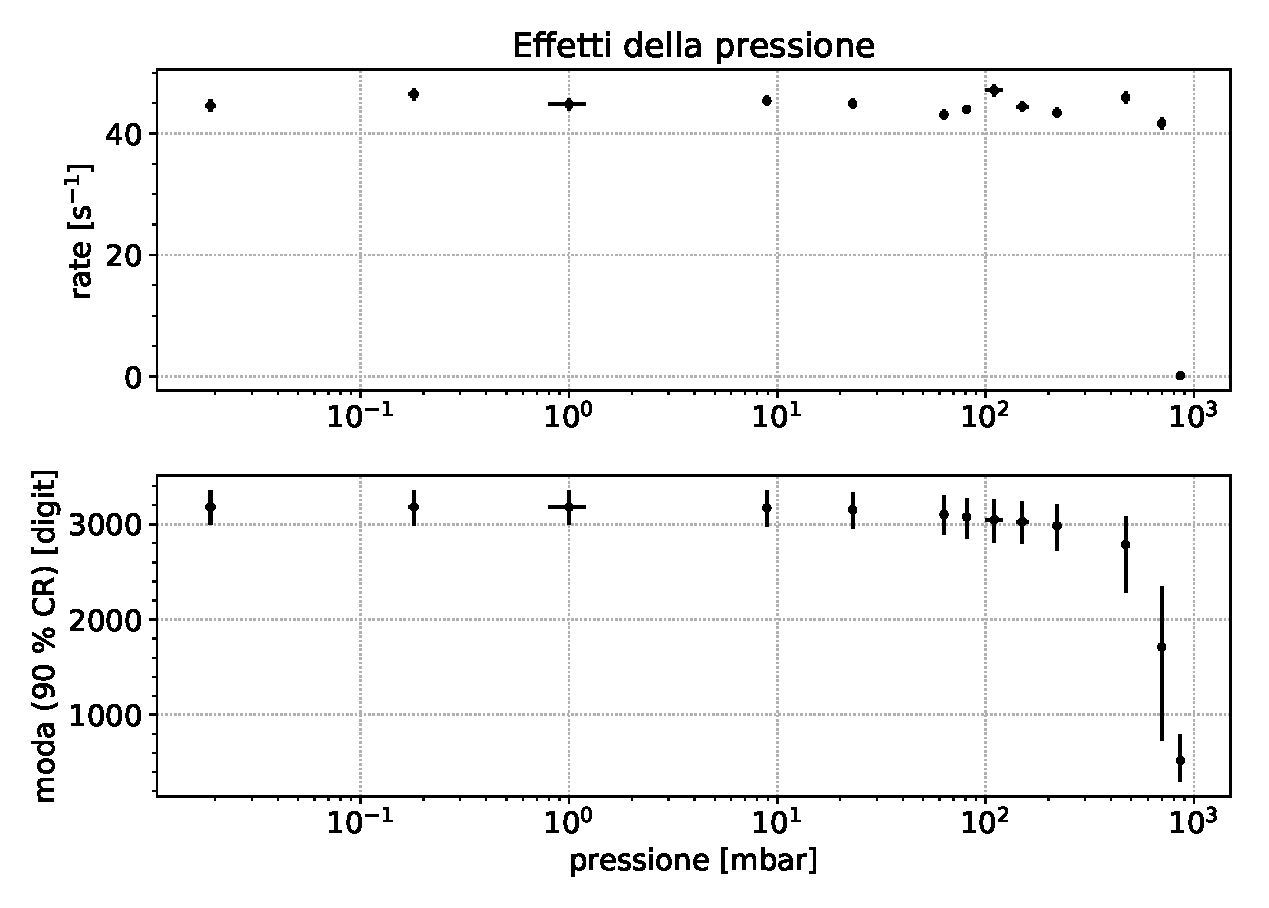
\includegraphics[width=\textwidth]{immagini/press}
\caption{Effetti della pressione su conteggi e spettri.
Il pannello superiore mostra il rate al variare della pressione,
quello sottostante la moda dello spettro,
dove le barre indicano la regione che contiene il \SI{90}\% dei campioni a massima densità.
La densità e la moda sono calcolate con una kernel density estimation (KDE).}
\label{fig:press}
\end{figure}
